\begin{figure}[!h]
    \centering
    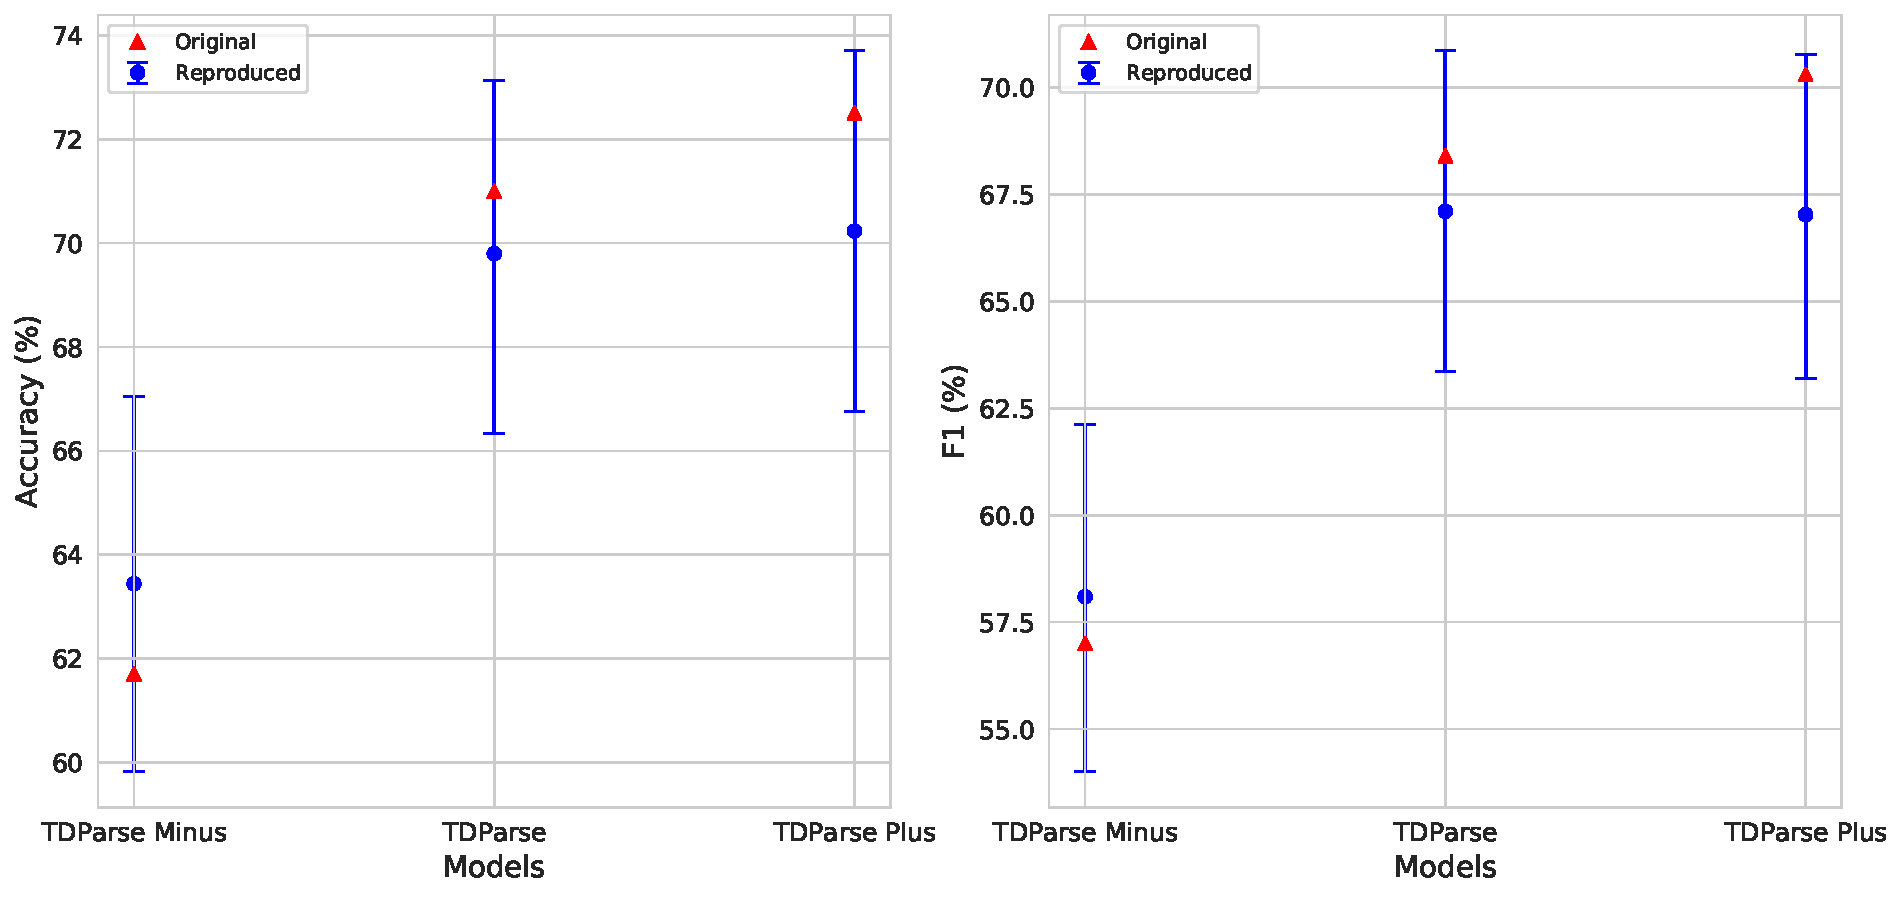
\includegraphics[scale=0.42]{images/reproducibility/wang/TDParse_F1_C_value_Dong.pdf}
    \caption{Using the C-values optimised for macro F1 metric, the confidence intervals for the two tailed test on the \citet{dong-etal-2014-adaptive} test set.}
    \label{fig:repro_wang_TDParse_Dong_macro_f1_c_values}
\end{figure}

\begin{figure}[!h]
    \centering
    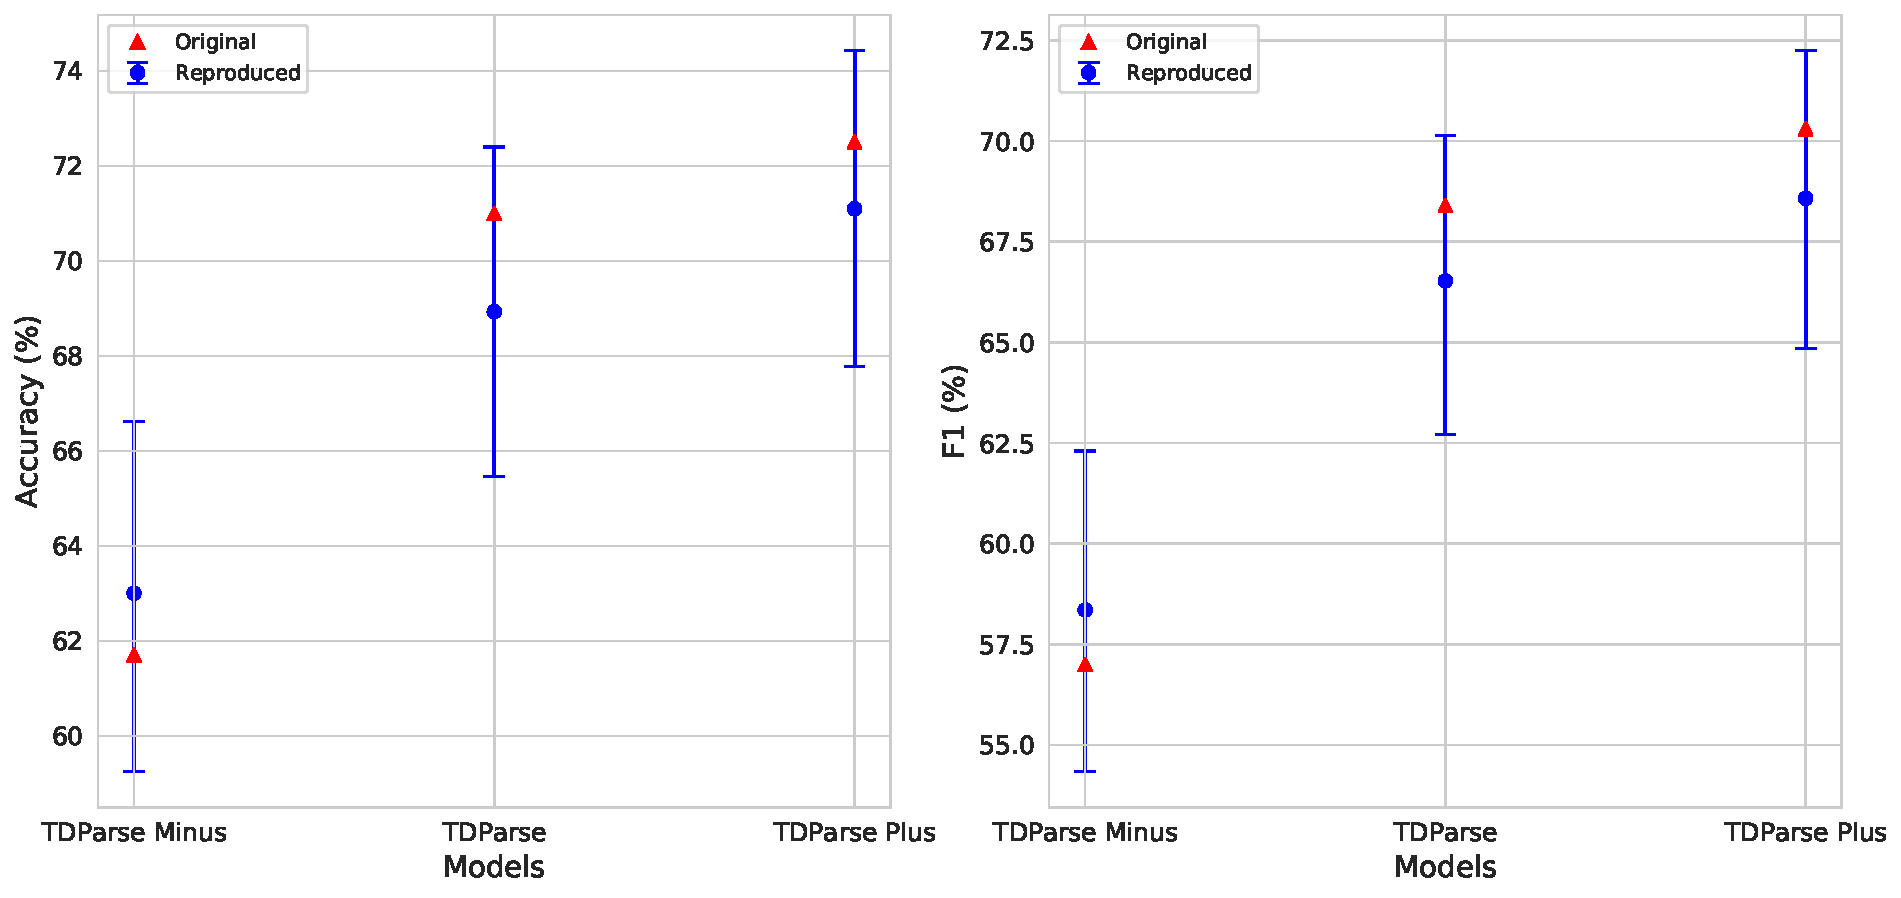
\includegraphics[scale=0.42]{images/reproducibility/wang/TDParse_F1_C_value_alt_scale_Dong.pdf}
    \caption{Using the C-values optimised for macro F1 metric with the original MinMax scaling range of \citet{wang-etal-2017-tdparse}, the confidence intervals for the two tailed test on the \citet{dong-etal-2014-adaptive} test set.}
    \label{fig:repro_wang_TDParse_Dong_alt_scaling_macro_f1_c_values}
\end{figure}

\begin{figure}[!h]
    \centering
    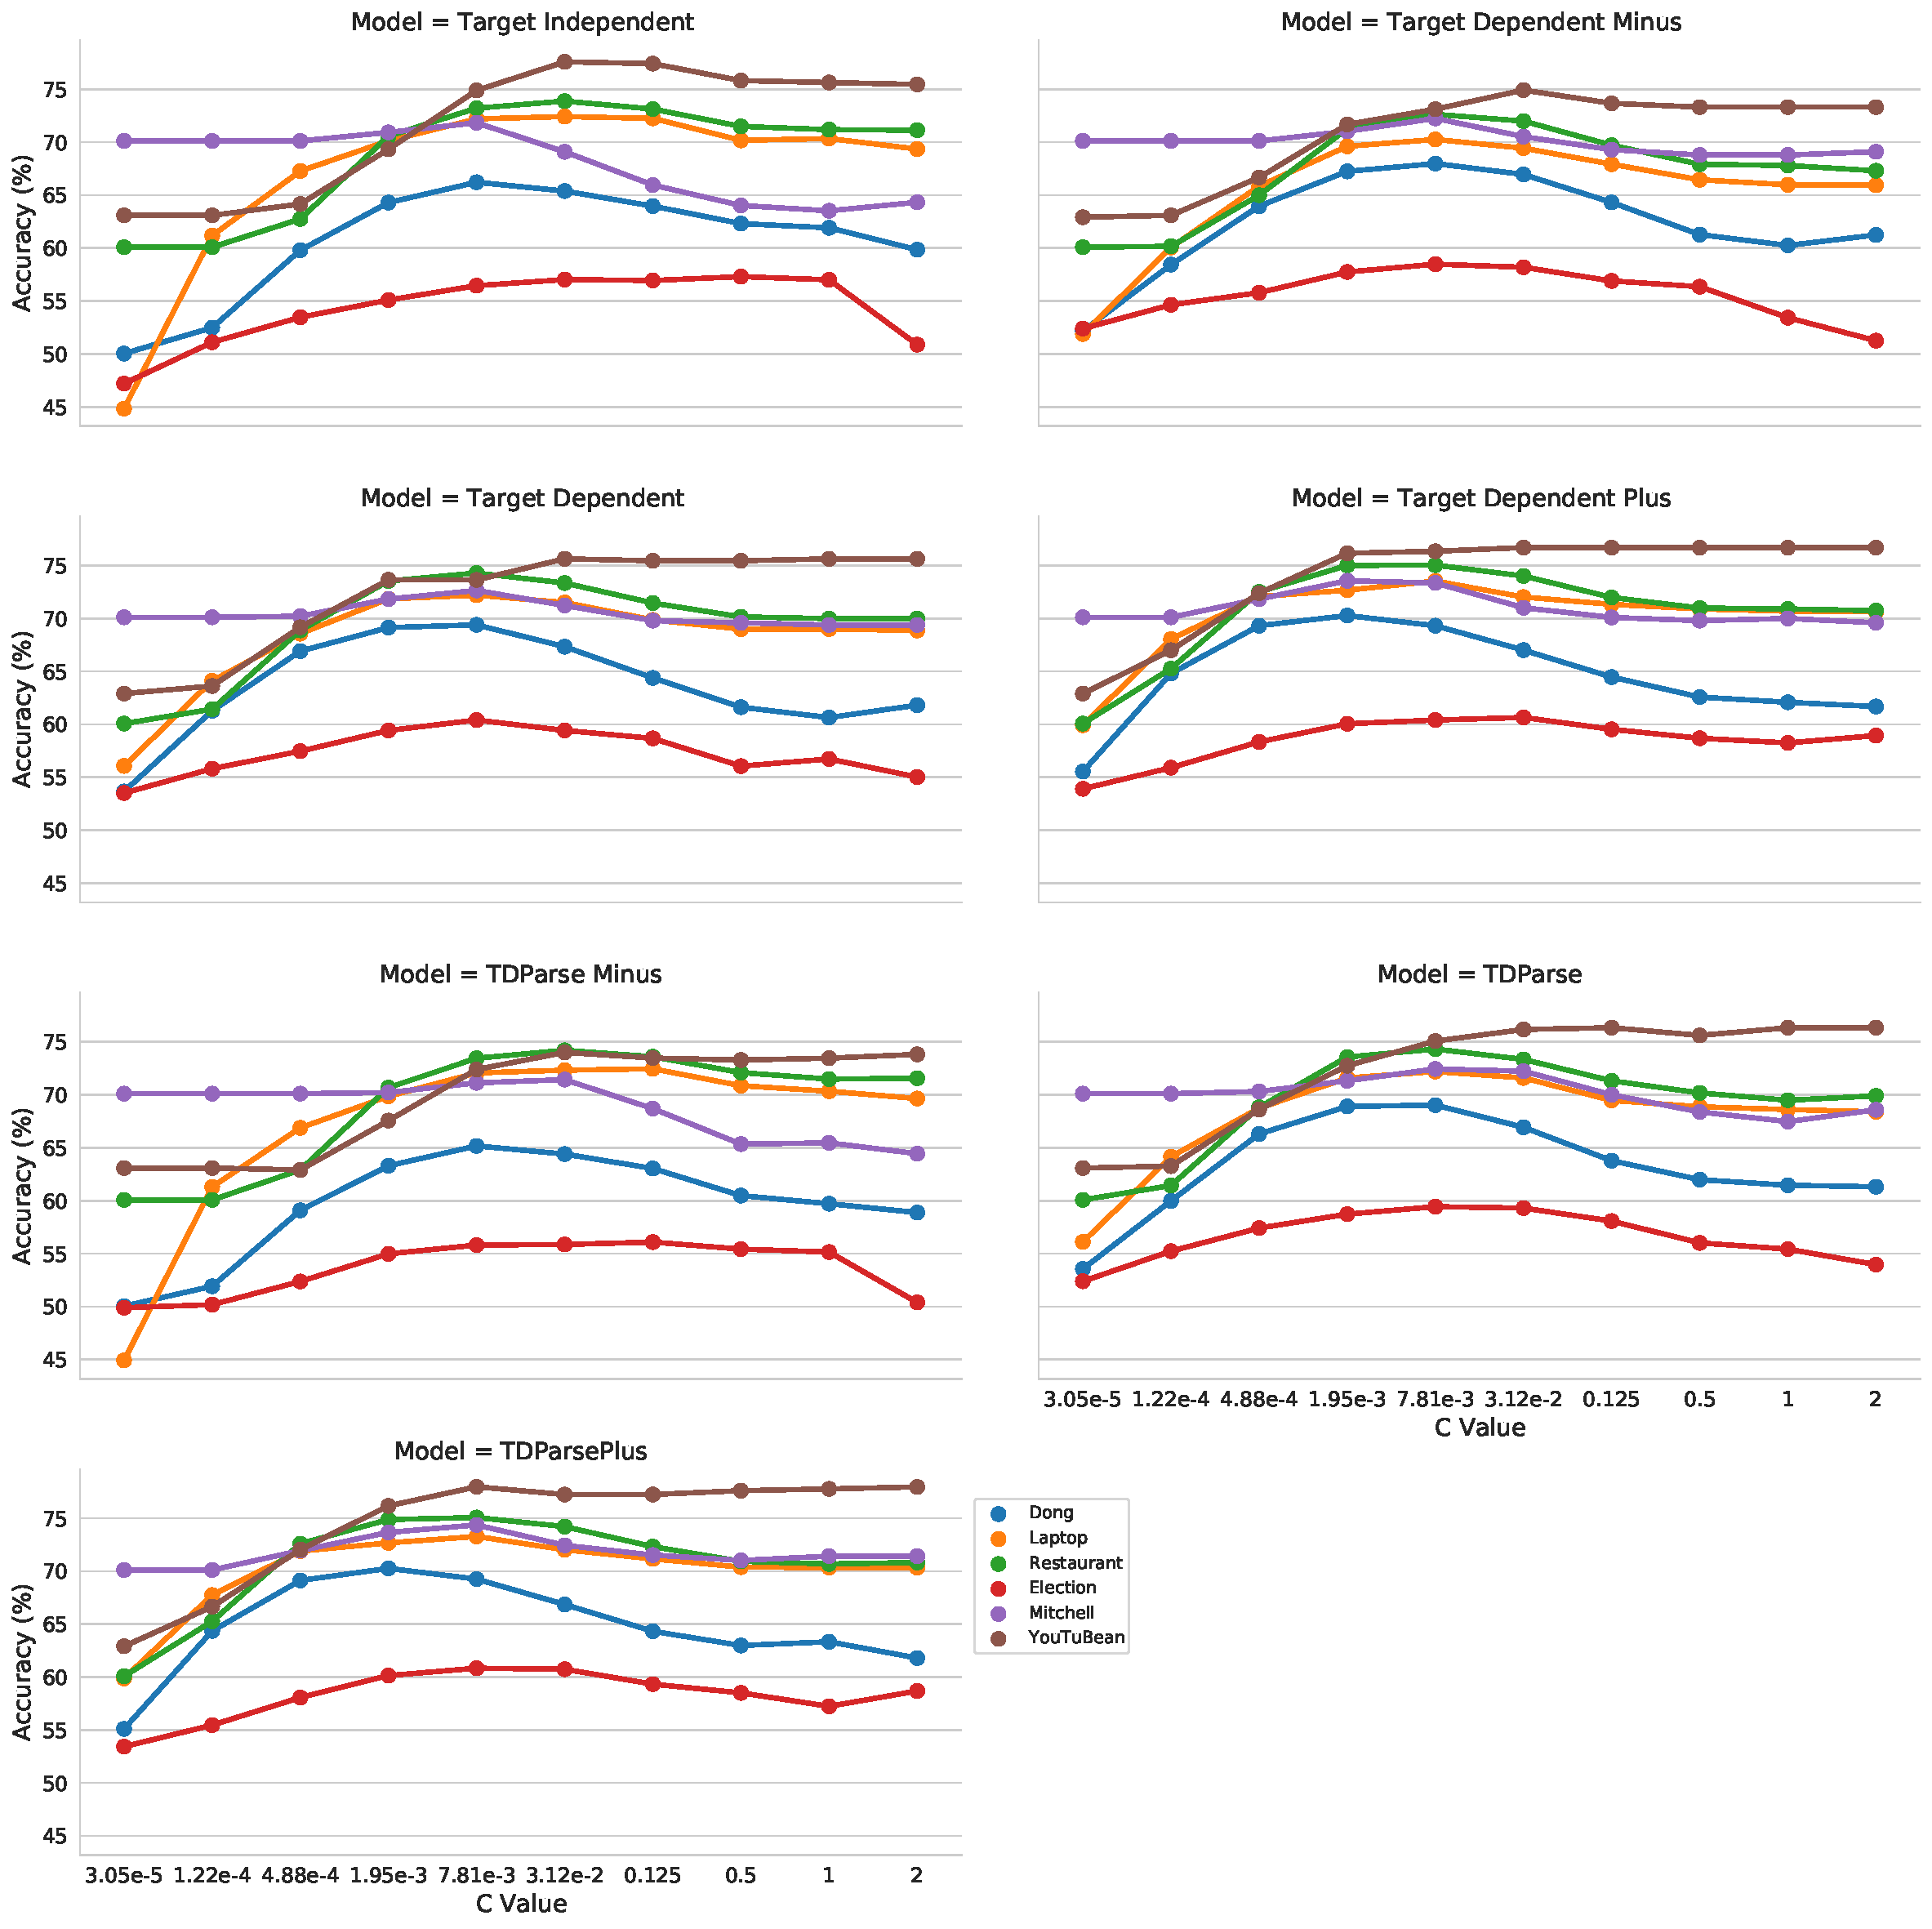
\includegraphics[scale=0.35]{images/reproducibility/Parameters/C_Value/C_Accuracy_Plot.pdf}
    \caption{The mean accuracy from five-fold cross validation on the training set for each C-value.}
    \label{fig:repro_parameters_c_accuracy_plot}
\end{figure}

\begin{figure}[!h]
    \centering
    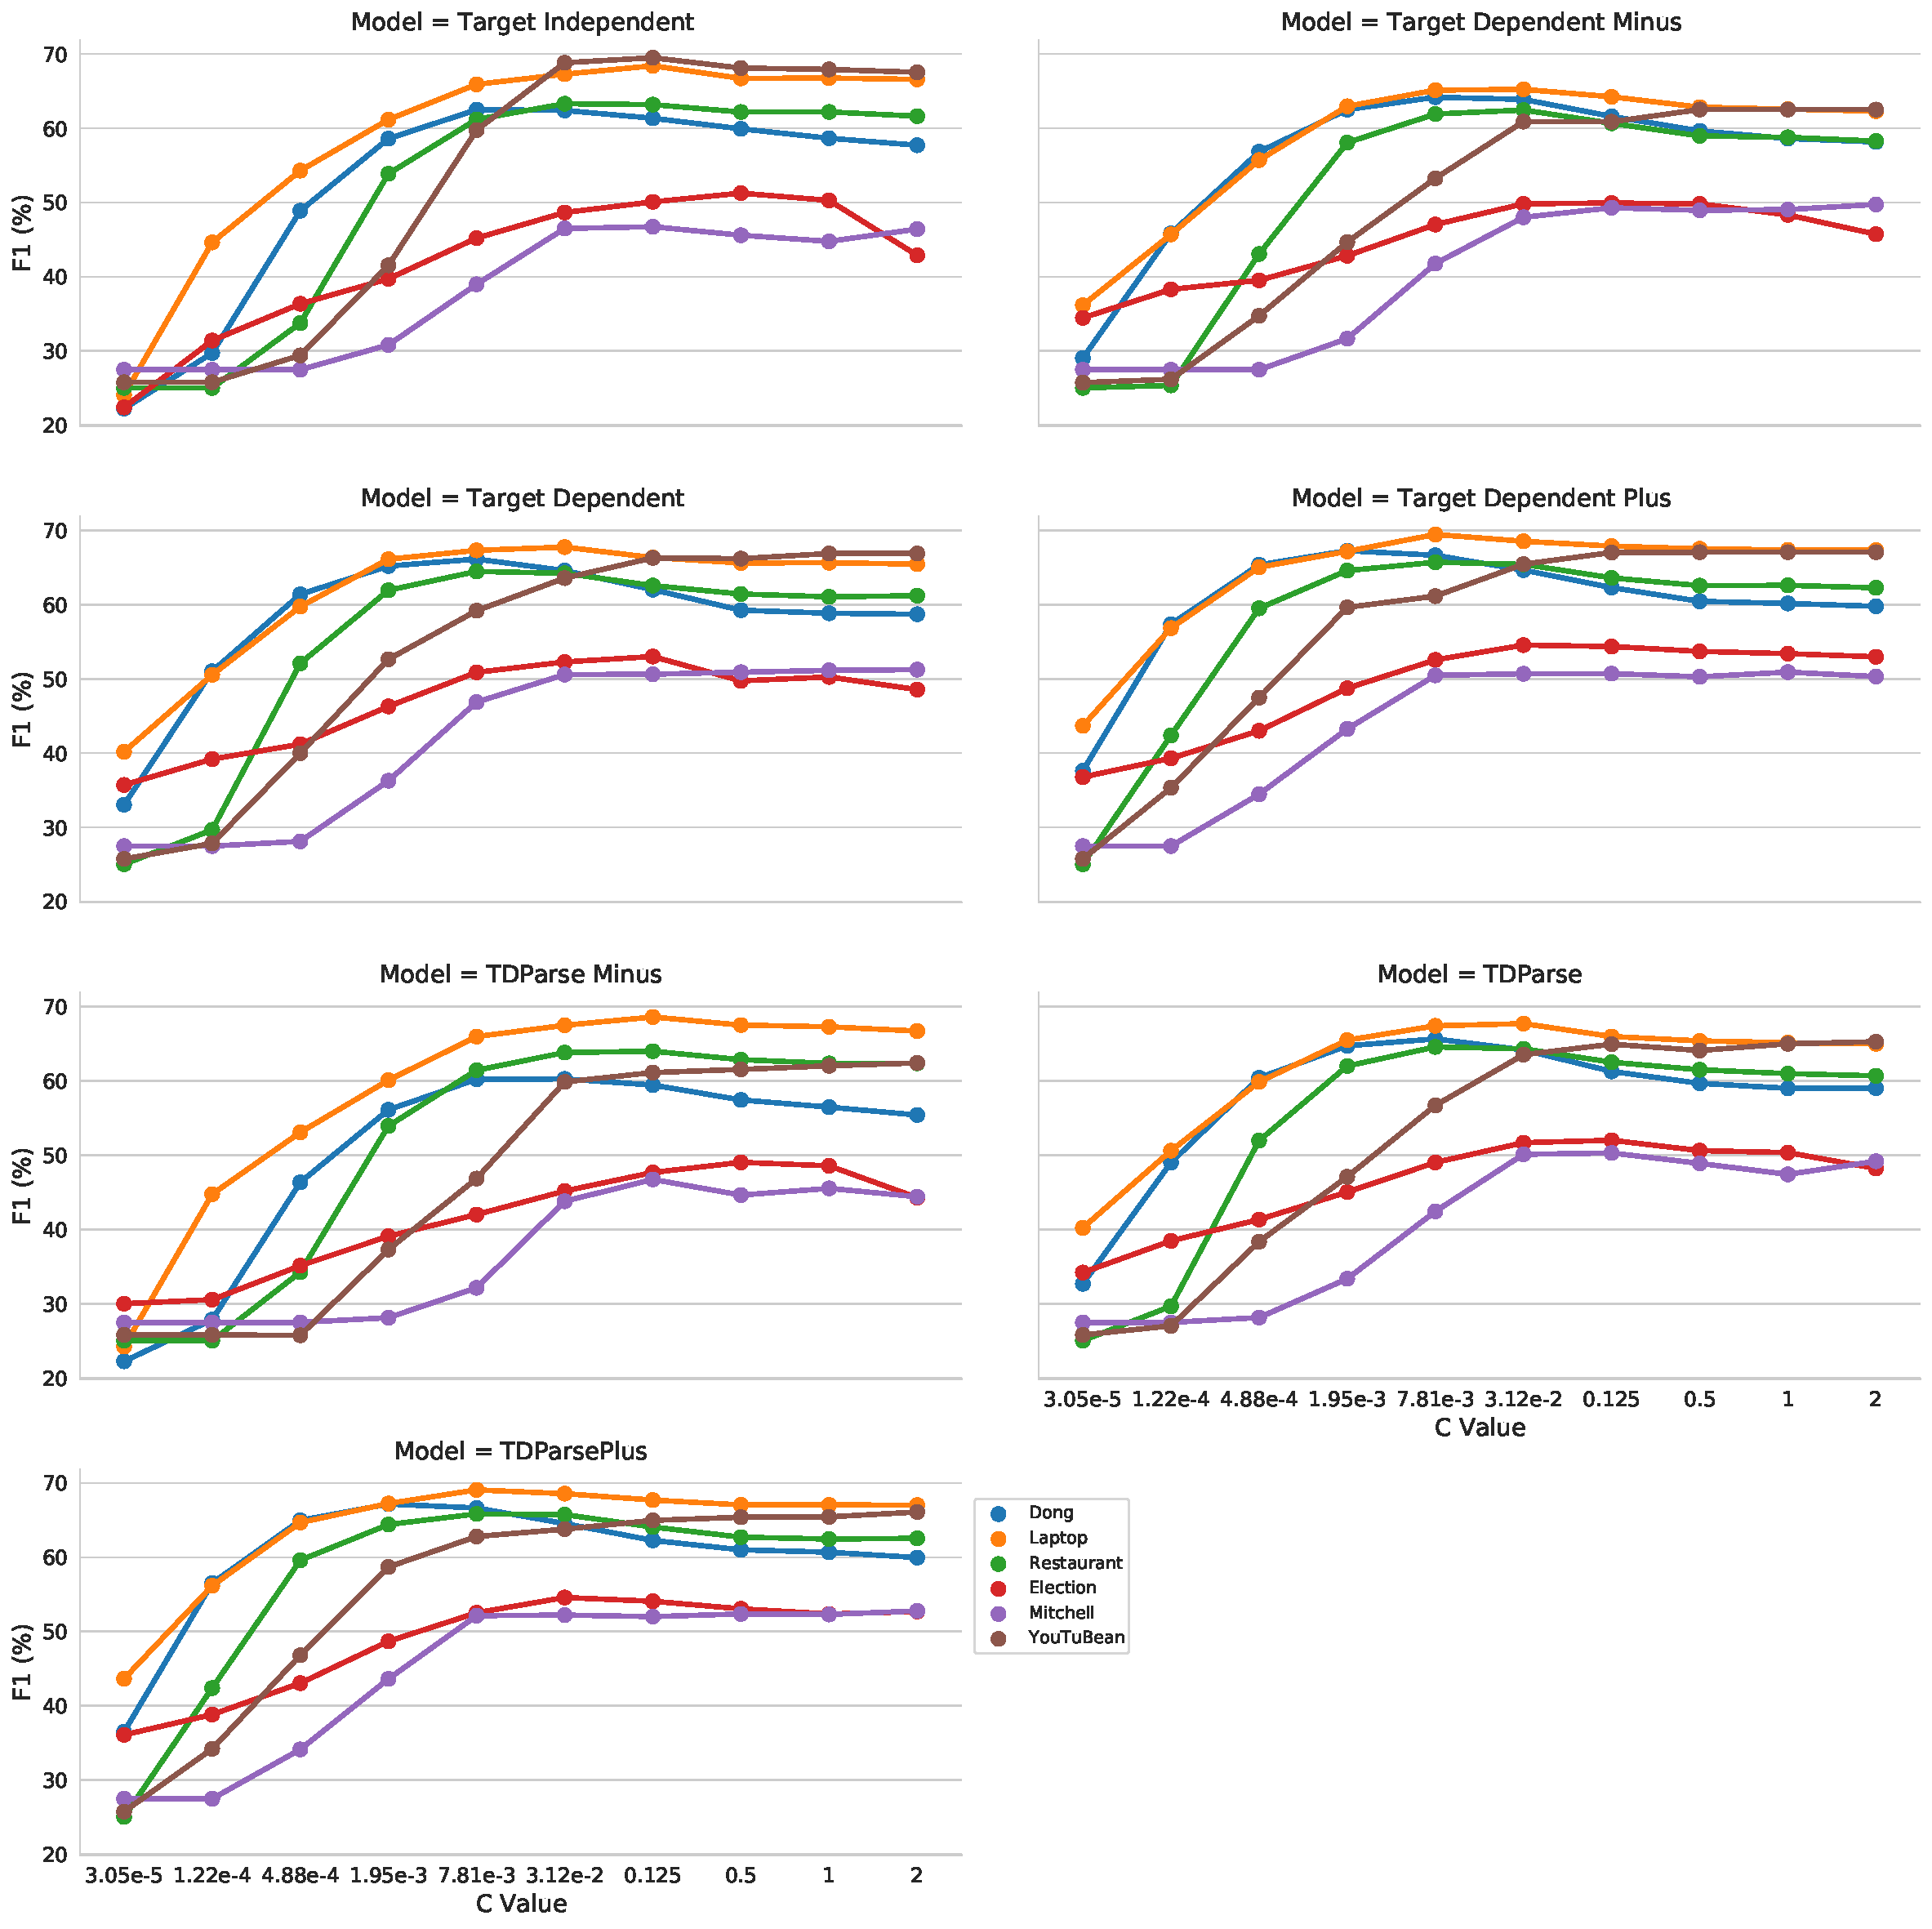
\includegraphics[scale=0.35]{images/reproducibility/Parameters/C_Value/C_F1_Plot.pdf}
    \caption{The mean macro F1 from five-fold cross validation on the training set for each C-value.}
    \label{fig:repro_parameters_c_macro_f1_plot}
\end{figure}

\begin{figure}[!h]
    \centering
    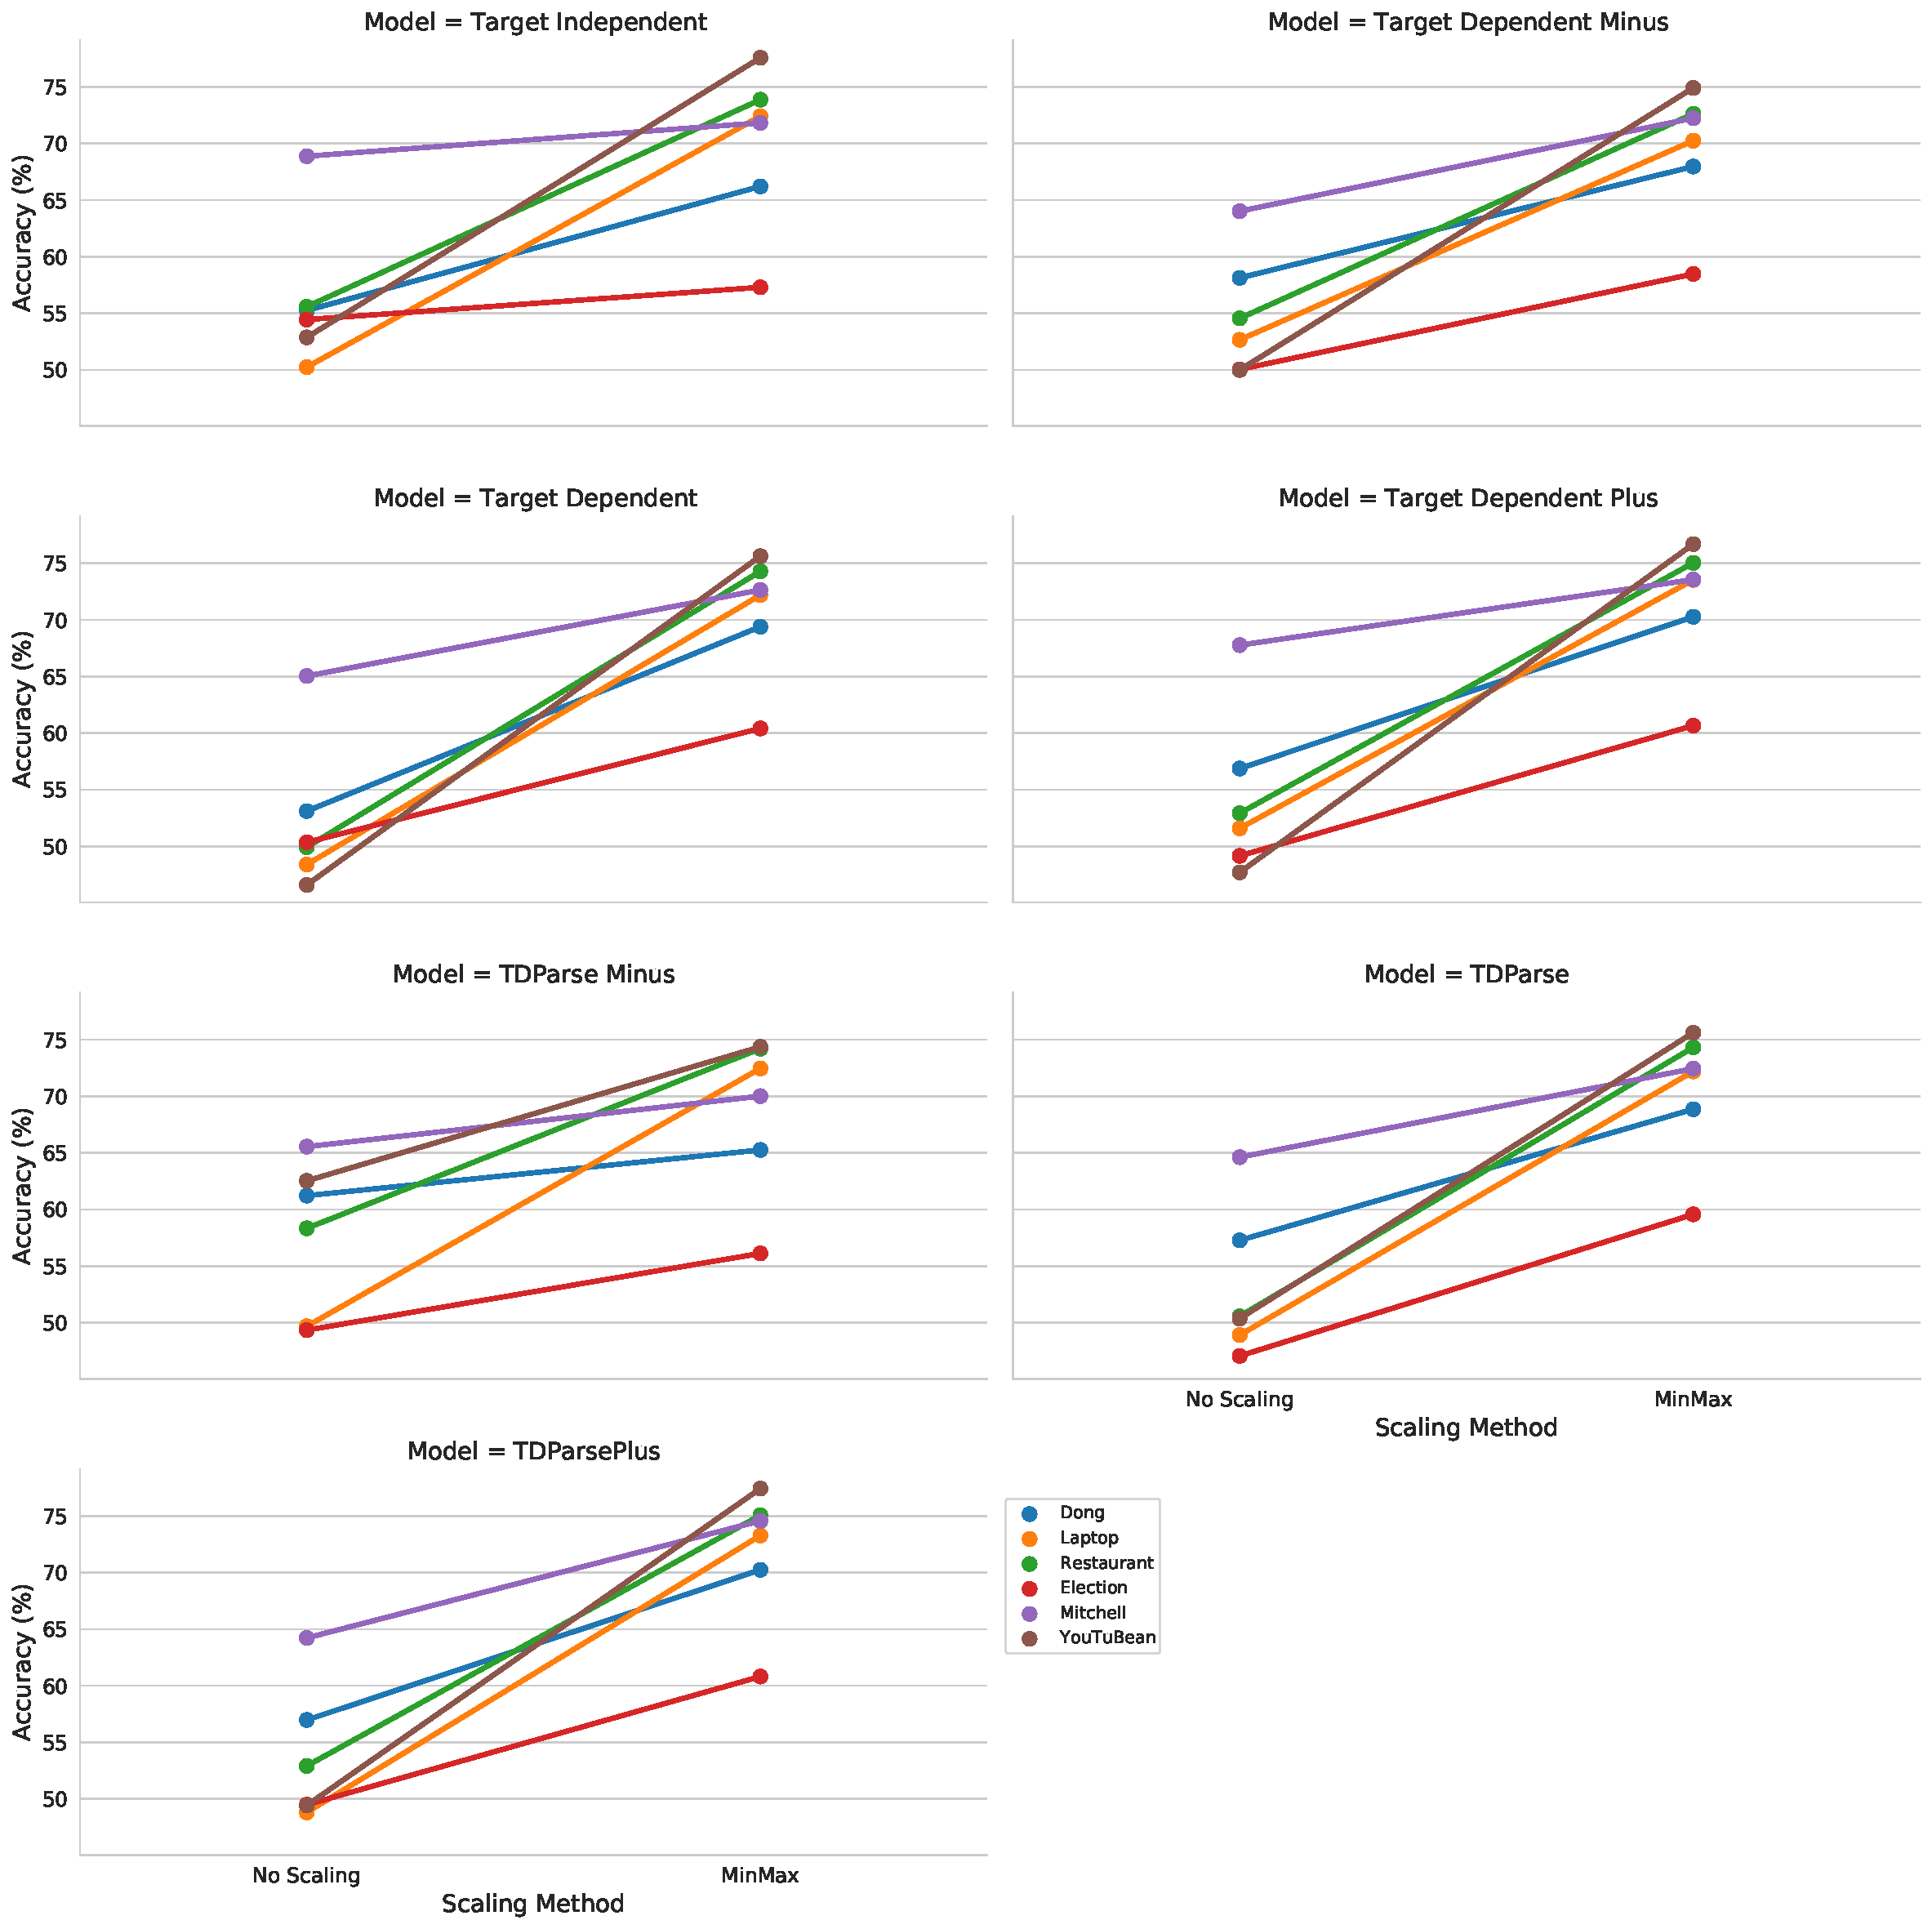
\includegraphics[scale=0.35]{images/reproducibility/Parameters/Scaling/Scaling_Accuracy_Plot.pdf}
    \caption{The mean accuracy from five-fold cross validation on the training set for the two scaling methods.}
    \label{fig:repro_parameters_scaling_accuracy_plot}
\end{figure}

\begin{figure}[!h]
    \centering
    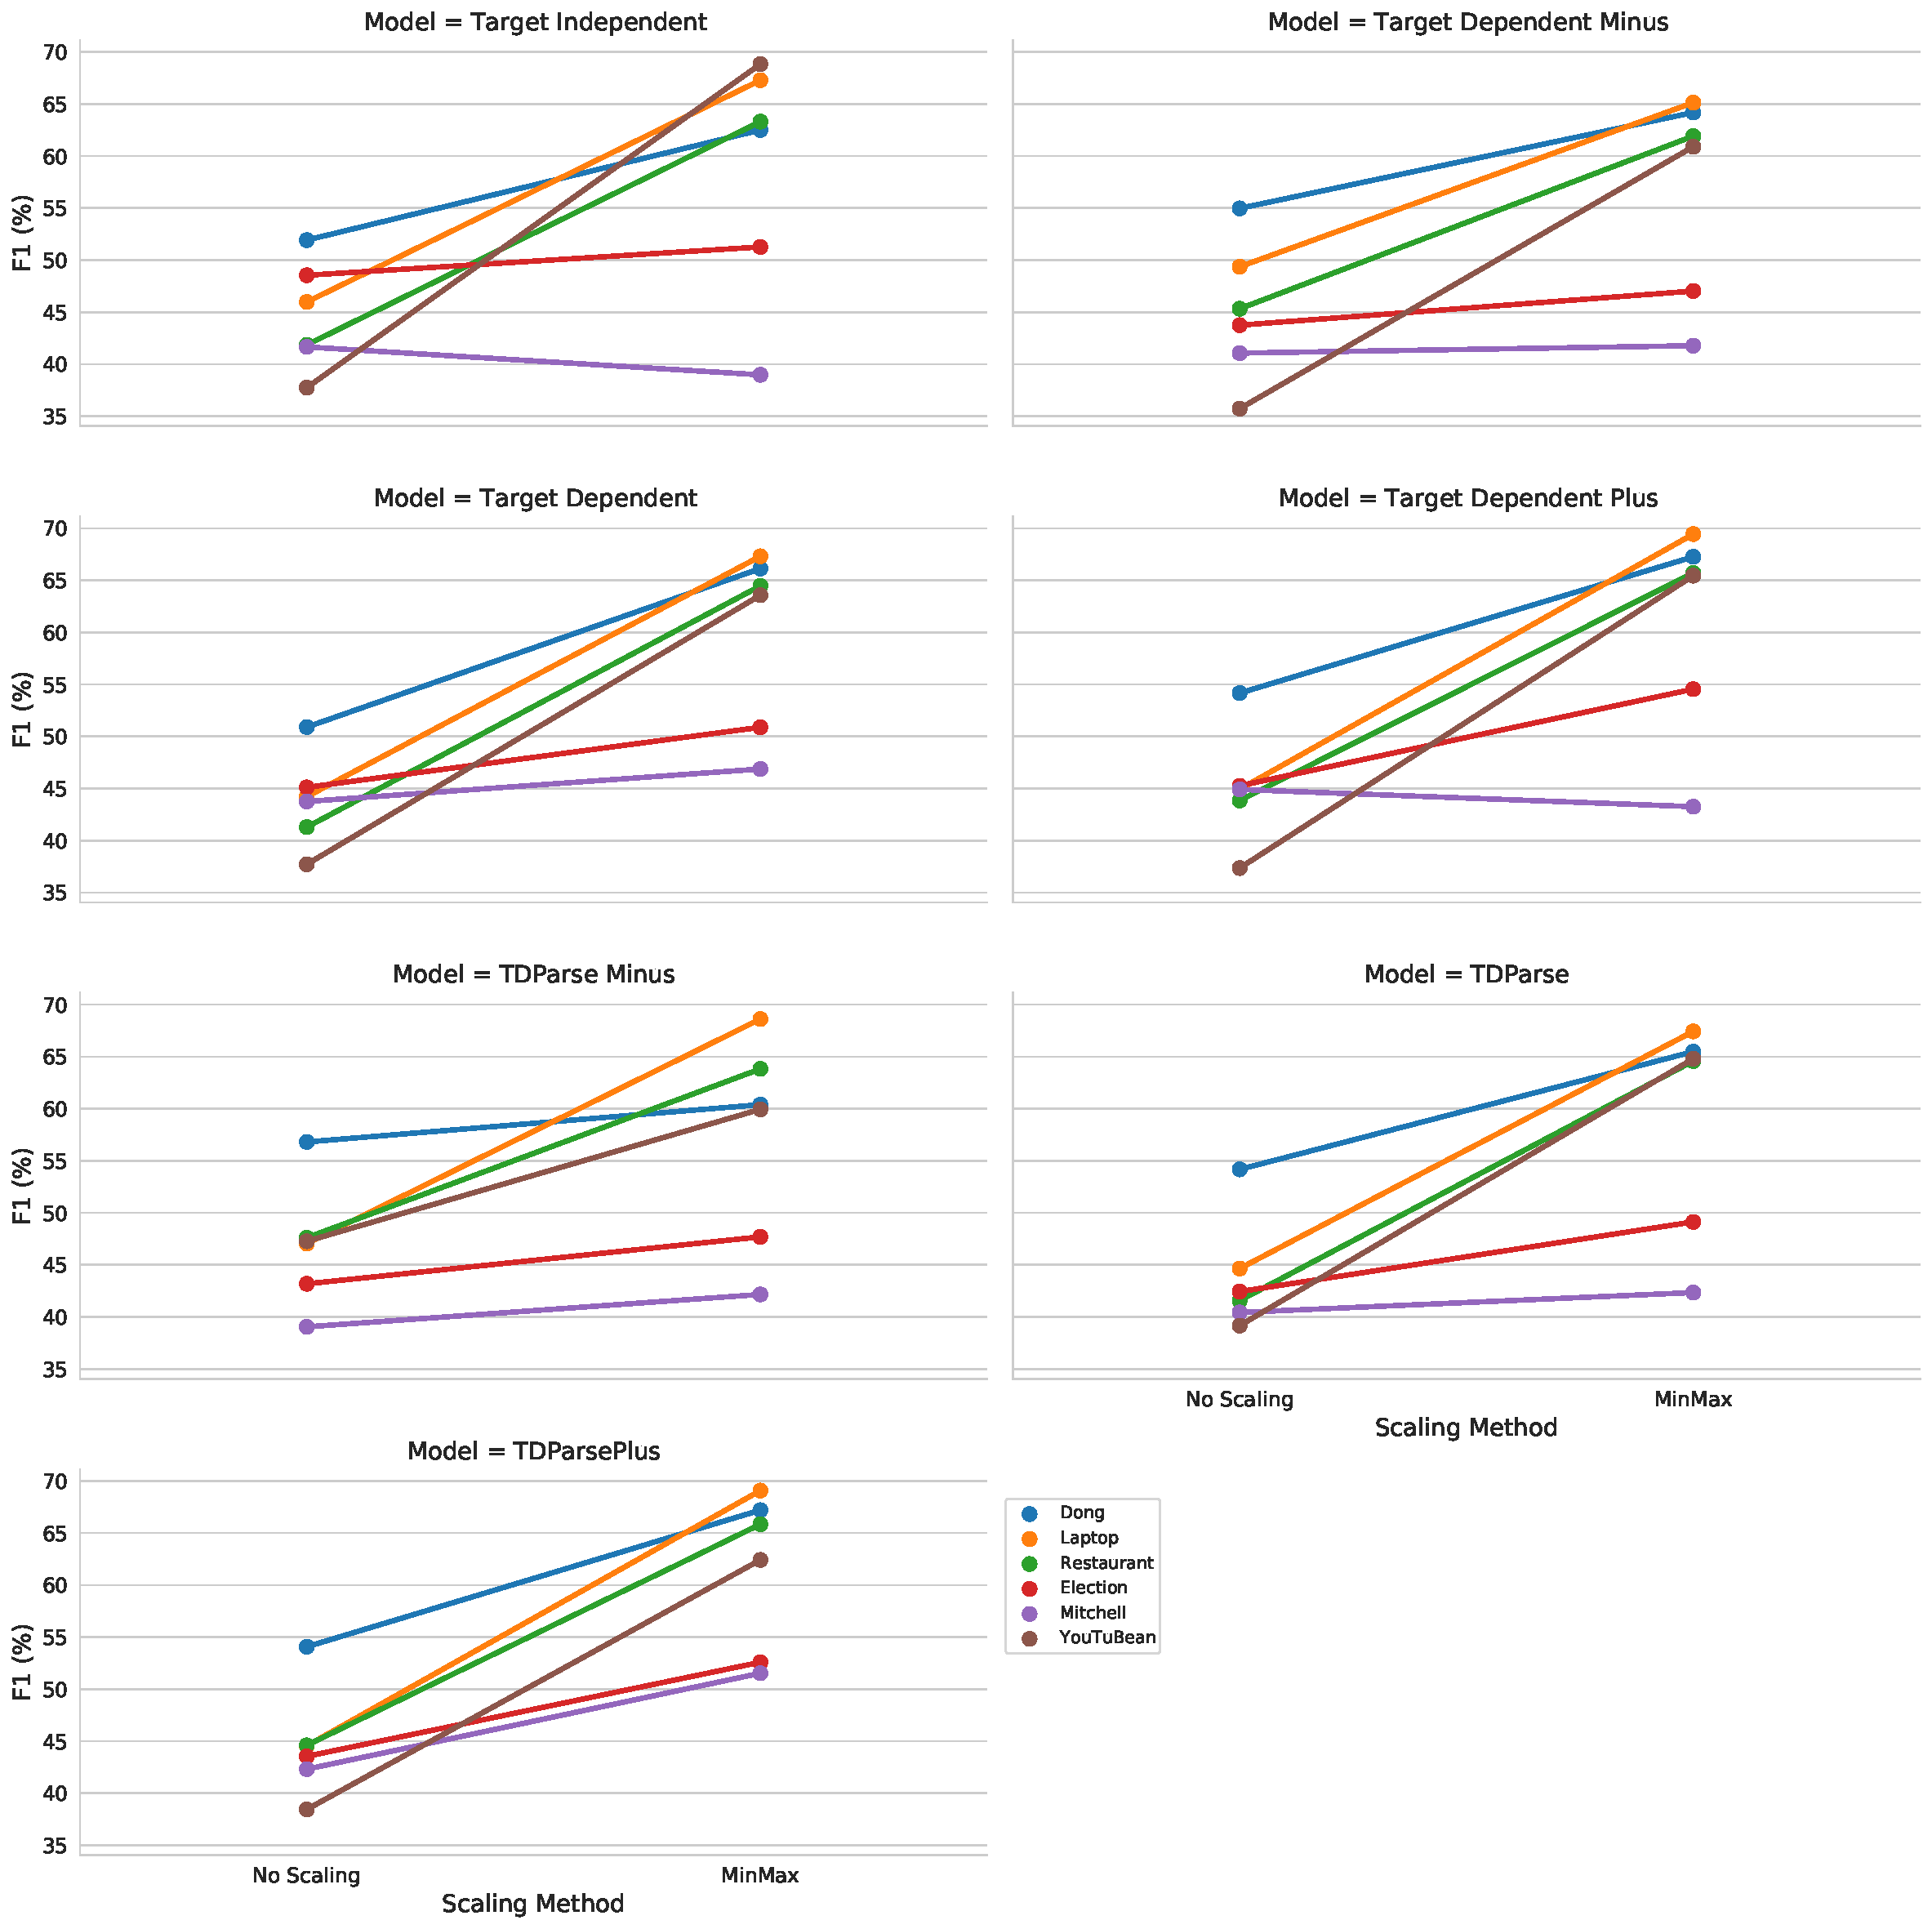
\includegraphics[scale=0.35]{images/reproducibility/Parameters/Scaling/Scaling_F1_Plot.pdf}
    \caption{The mean macro F1 from five-fold cross validation on the training set for the two scaling methods.}
    \label{fig:repro_parameters_scaling_macro_f1_plot}
\end{figure}

\begin{figure}[!h]
    \centering
    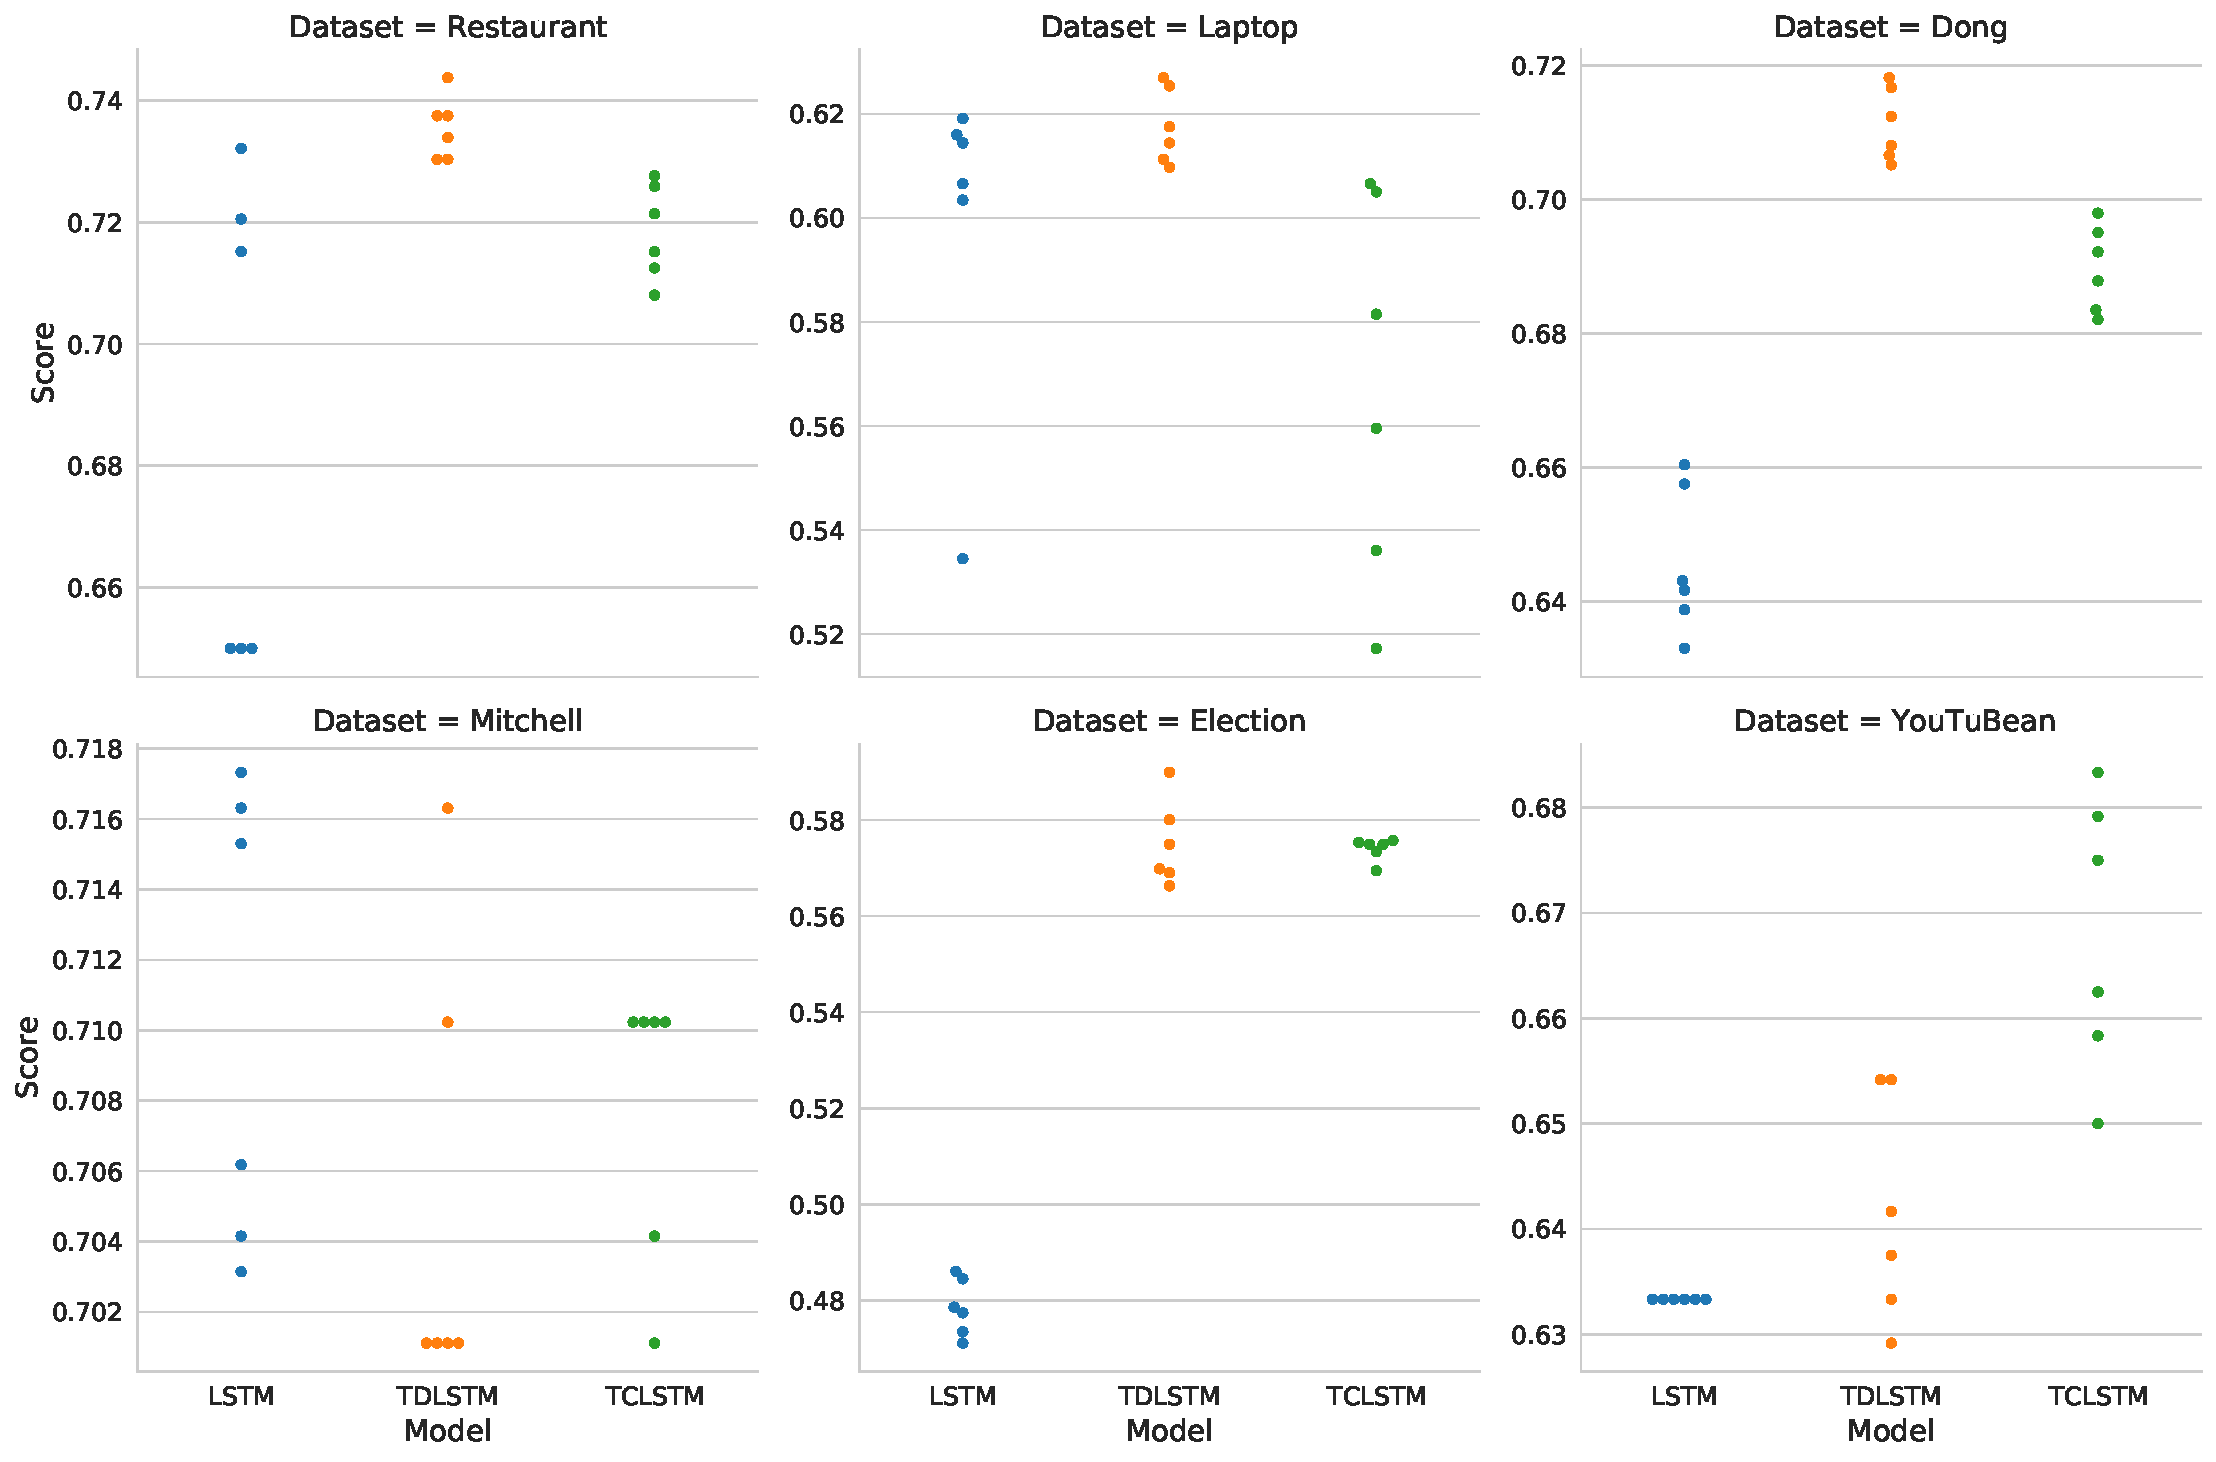
\includegraphics[scale=0.35]{images/reproducibility/LSTM_Test_ACC.pdf}
    \caption{Distribution of accuracy scores from the six runs for each LSTM method and test dataset.}
    \label{figure:repro_LSTM_TEST_ACC}
\end{figure}